\PassOptionsToPackage{dvipsnames}{xcolor}
\documentclass[serif,envcountsect,table,t%, handout
]{beamer}%
\usepackage{amsmath, animate, hyperref, subcaption, tikz, multirow}
\usetheme{CambridgeUS}
\usecolortheme{wolverine}
\usecolortheme{orchid}
\setbeamertemplate{navigation symbols}{}
\graphicspath{{../figures/}}
\usetikzlibrary{shapes,shadows}
\addtobeamertemplate{frametitle}{}{\vspace{-3mm}} % reduce top space
\setbeamertemplate{caption}[numbered] 
%%%%----------------------------------------------------------
\begin{document}
\title[Probability and Paradoxes]{Pre College Summer -- Data Science\\
Probability: Intuition and Paradoxes}
\author[Bar, Wang]{Haim Bar, HaiYing Wang}
\date[]{}
\institute[UConn]{\normalsize University of Connecticut}
%%%% -------------------------------------------------
\begin{frame}[noframenumbering] \titlepage \end{frame}
%%%% -------------------------------------------------
\begin{frame}{Randomness}
  \begin{center}
    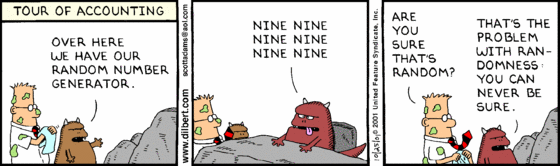
\includegraphics[width=\textwidth]{random.png}
  \end{center}
  \begin{itemize}
  \item The world is random. Probability theory has been developed to quantify
    the randomness.
  \item We will go through examples to see how probability helps interpret
    phenomena in real life and how probability may counter intuition.
  \end{itemize}
\end{frame}
%%%% ---------------------------------------------------------
\begin{frame}{Some concepts:}
\begin{itemize}
\item \emph{Experiment}: a situation in which the outcome occurs randomly, e.g.,
  flipping a coin, rolling a dice, and picking a card from a deck.
\item \emph{Sample Space}: the set of all possible outcomes in an experiment, e.g.,
  \{head, tail\}, \{1, 2, ..., 6\}, and \{all card faces\}.
\item \emph{Event}: a subset of the sample space is called an event; an event
  occurs if the outcome from an experiment belong to the subset. For example, if
  you roll a die, and you are interested in the result of having an even number,
  then the event is $E$=\{2, 4, 6\}.
\end{itemize}
\begin{figure}[htbp]
\centering
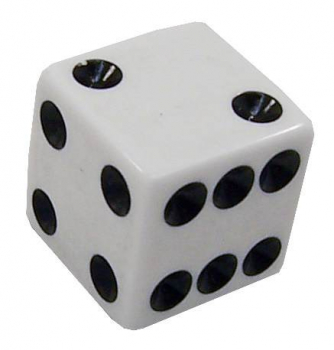
\includegraphics[width=0.2\textwidth]{die.jpg}\hspace{9mm}
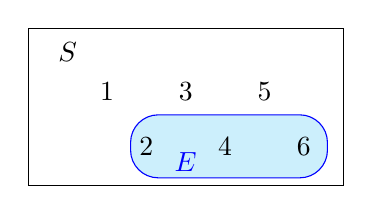
\begin{tikzpicture}
  \draw (-2, 2) rectangle (2, 0);
  \draw[rounded corners=10pt, fill = cyan!20, draw=blue] (-0.7,0.1) rectangle ++(2.5,0.8);
  \draw (-1.5, 1.7) node{$S$};
  \draw (-1, 1.2) node{1} (0, 1.2) node{3} (1, 1.2) node{5};
  \draw (-0.5, 0.5) node{2} (0.5, 0.5) node{4} (1.5, 0.5) node{6};
  \draw[text = blue] (0, 0.3) node{$E$};
\end{tikzpicture}
\caption{Sample space (the outcomes of a fair six-sided die) and event (rolling an even number) illustrated with Venn diagram. }
\label{fig:probability-event}
\end{figure}
\end{frame}
%%%% ---------------------------------------------------------
\begin{frame}{Probability}
\begin{itemize}
\item \emph{Probability} is a number between zero and one which tells us how
  likely an event to occur. If we assume each possible outcome in an experiment has an equal chance to
  occur, then the probability of event $E$ is
  \begin{equation}
    P(E) =\frac{\text{size of } E}{\text{size of } S}.
  \end{equation}
% \item Note that this formula
%   holds only if all the outcomes are equally likely.
\item In the example in Figure~\ref{fig:probability-event}, the probability that
we roll an even number when we use a fair die, is
$$P(even)=\frac{3}{6}=0.5$$.
% \item In the following chapters we will deal with infinite (even uncountable) sample spaces, and we will generalize the definition of $P(E)$ then.
\end{itemize}
\end{frame}
%%%%----------------------------------------------------------
\begin{frame}% [<+-| alert@+>]
  {Example: Cards}
\begin{itemize}
\item Experiment: Shuffle a standard 52 card deck and choose one card
\item Sample Space:\\[3mm]
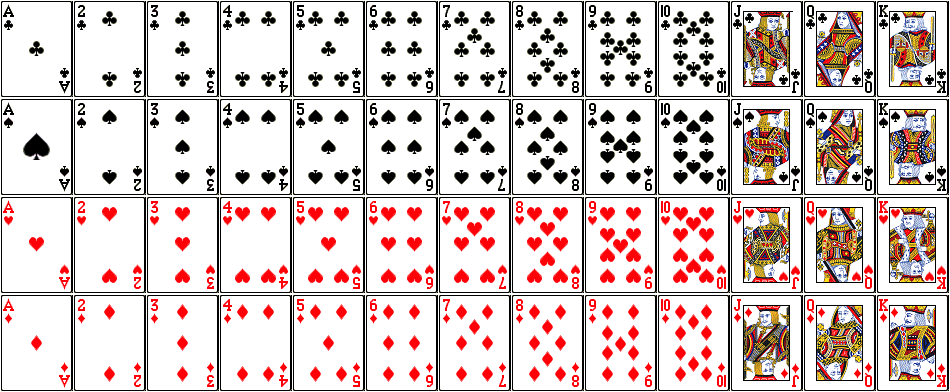
\includegraphics[width=0.95\textwidth]{cards.png}
\end{itemize}
\end{frame}
%%%%----------------------------------------------------------
\begin{frame}% [<+-| alert@+>]
  {Example: Cards}
\begin{itemize}
% \item Event: Each card is a simple event. There are 52 simple events.
\item Event: Get a face card.\\[2mm]
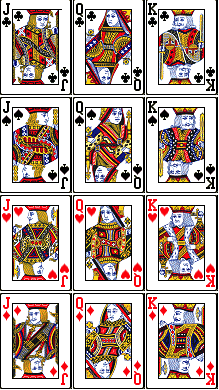
\includegraphics[width=0.27\textwidth]{cards2.png}
\item The probability of getting a face card?
\end{itemize}
\end{frame}
%%%%----------------------------------------------------------
\begin{frame}{Elevator waiting time}
  Mr. Smith works on the 13th floor of a 15 floor building. The only elevator
  moves continuously through floors 1, 2, . . . 14, 15, 14, . . . 2, 1, 2,
  . . . , except that it stops on a floor on which the button has been
  pressed. Assume that time spent loading and unloading passengers is very small
  compared to the travelling time.  Mr.~Smith complains that at 5pm, when he
  wants to go home, the elevator almost always goes up when it stops on his
  floor. What is the explanation?
\end{frame}
%%%%----------------------------------------------------------
\begin{frame}{Intransitive Dice}
  \begin{itemize}
  \item Real numbers are transitive, meaning that if we know that $x>y$ and
    $y>z$ then $x>z$.
  \item However, probabilities of events are not always transitive.
  \item This may be more aligned with real life. For example, consider three
    tennis players, say Alice, Bella, and Claire.
    \begin{itemize}
    \item Alice wins Bella more frequently;
    \item Bella wins Clair more frequently;
    \item does Alice win Clair more frequently?
    \end{itemize}
  \end{itemize}
\end{frame}
%%%% ----------------------------------------------------------
\begin{frame}{Intransitive Dice}
Consider three dice with different sides numbers:
\begin{itemize}
\item Die A has sides 2, 2, 4, 4, 9, 9.
\item Die B has sides 1, 1, 6, 6, 8, 8.
\item Die C has sides 3, 3, 5, 5, 7, 7.
\end{itemize}
To play a game using dice A and B, you can chose which die to roll and your
opponent rolls the other. The one who tolls a larger number wins. Which die do
you want to choose? How about B v.s. C? \pause
\begin{center}\small
  \begin{tabular}{cc|ccc}\hline
    &   & \multicolumn{3}{c}{B} \\
    % \cline{3-5}
    &   & 1                & 6                & 8                \\ \hline
    \multirow{3}{*}{A}
    & 2 & \color{red}$A>B$ & $A<B$            & $A<B$            \\
    & 4 & \color{red}$A>B$ & $A<B$            & $A<B$            \\
    & 9 & \color{red}$A>B$ & \color{red}$A>B$ & \color{red}$A>B$ \\\hline
  \end{tabular}
  \hspace{.2cm}
  \begin{tabular}{cc|ccc}\hline
    &   & \multicolumn{3}{c}{B} \\
    % \cline{3-5}
    &   & 1                & 6                & 8                \\ \hline
    \multirow{3}{*}{C}
    & 3 & \color{red}$C>B$ & $C<B$            & $C<B$            \\
    & 5 & \color{red}$C>B$ & $C<B$            & $C<B$            \\
    & 7 & \color{red}$C>B$ & \color{red}$C>B$ & $C<B$ \\\hline
  \end{tabular}
\end{center}
\end{frame}
%%%%----------------------------------------------------------
\begin{frame}{Conditional Probability}
  \begin{itemize}
  \item When there are two events $A$ and $B$ under consideration, knowing that
    $A$ has occurred may change the probability for $B$ to occur.
  \item This is called the \emph{conditional probability} of $B$ given $A$,
    often written as $P(B\mid A)$.
  \item Two events $A$ and $B$ are \emph{independent} if $P(B\mid A) = P(B)\,.$
\end{itemize}
   % For example, suppose that someone rolls a die behind a curtain and tells us
   % only that the number is less than or equal to 3. What is the probability that
   % it is an even number?
   % iven that we got 1, 2, or 3, the only possibility that
   % it is even is if the number is 2.
% The \emph{unconditional} probability of getting an even number in a roll of
% a die is 1/2, but because of the information that provided to us, we conclude
% that the \emph{conditional} probability is 1/3.
   
% Using mathematical notation, we write  $P(B\mid A)=1/3$ which stands for ``conditional on $A$=the number is less than or equal to 3, the probability of $B$=the number is even, is 1/3''. 

% Once again, it is helpful to visualize such things using a Venn diagram. In Figure~\ref{fig:probability-conditional}, the sample space $S$ consists of the six possible outcomes and the two events are depicted as a circle (event $A$) and as a rounded rectangle ($B$). To say that we condition on $A$ means that we restrict our view and look only at outcomes that could occur if we are told that $A$ has occurred. In other words, our sample space becomes $A$, instead of the whole set, $S$.

\begin{figure}[htbp]
\centering
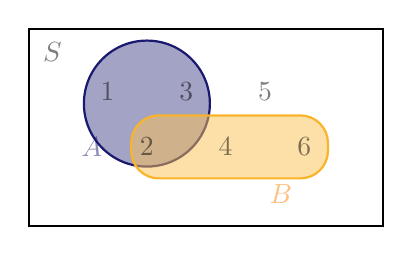
\begin{tikzpicture}[thick,fill opacity=0.5]
  \draw (-2, 2) rectangle (2.5, -0.5);
\draw[fill=MidnightBlue!80, draw=MidnightBlue] (-0.5, 1.05) circle (0.8);
  \draw[rounded corners=10pt, fill = Dandelion!80, draw=Dandelion] (-0.7,0.1) rectangle ++(2.5,0.8);
  \draw (-1.7, 1.7) node{$S$};
  \draw (-1, 1.2) node{1} (0, 1.2) node{3} (1, 1.2) node{5};
  \draw (-0.5, 0.5) node{2} (0.5, 0.5) node{4} (1.5, 0.5) node{6};
  \draw[text = orange] (1.2, -0.1) node{$B$};
  \draw[text = MidnightBlue] (-1.2, 0.5) node{$A$};
\end{tikzpicture}
\caption{Conditional probability -- given that we are told that a die gave a number less than or equal to 3 (event $A$), what is the probability that we got an even number ($B$)?}
\label{fig:probability-conditional}
\end{figure}

\end{frame}
%%%%----------------------------------------------------------
\begin{frame}{Two Children Problem}
Consider the following two problems:
\begin{enumerate}
\item Mr. Jones has two children. The older child is a girl. What is the
  probability that both children are girls?
\item Mr. Smith has two children. At least one of them is a girl. What is the
  probability that both children are girls?
\end{enumerate}
\end{frame}
%%%%----------------------------------------------------------
\begin{frame}{Bertrand's Box}
There are three boxes, one contains two gold coins, one contains two
silver coins, and one contains a gold coin and a silver coin.
A box is selected at random and a coin is taken from that box at random. If the
coin is a gold coin, what is the probability that the other coin in that box is
also a gold coin.
\end{frame}
%%%% ---------------------------------------------------------
\begin{frame}{Bertrand's Box}
  \begin{figure}[H]
\resizebox{0.9\columnwidth}{!}{%
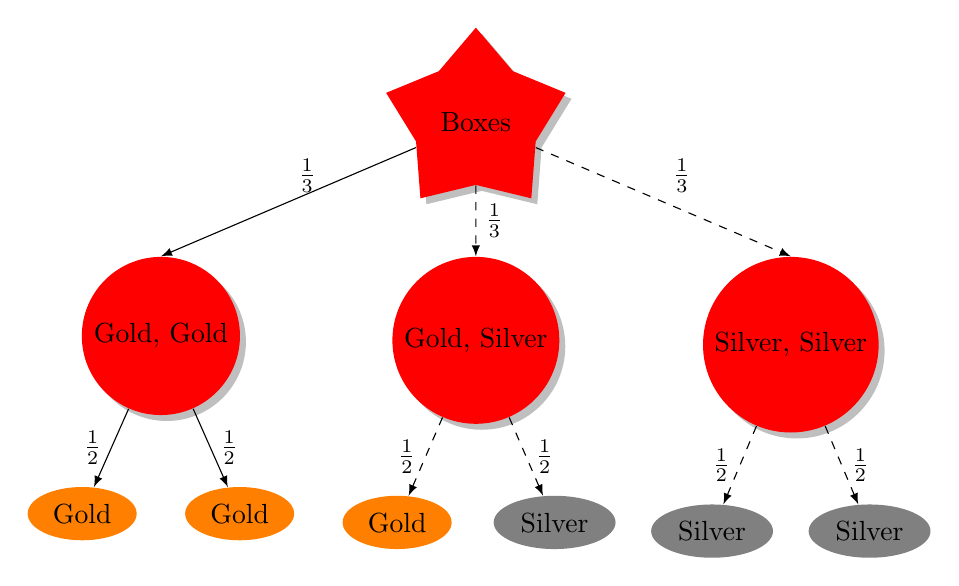
\begin{tikzpicture}[%scale=0.5,
  edge from parent/.style={draw,-latex},
    boxes/.style={star, draw=none, fill=red, drop shadow, text centered, anchor=north},
    state/.style={draw=none, fill=red, circle, drop shadow, text centered, anchor=north},
    leaf/.style={draw=none, fill=orange, ellipse, text centered, anchor=north},
    leafs/.style={draw=none, fill=gray, ellipse, text centered, anchor=north},
    level distance=0.9cm, growth parent anchor=south
]
\node [boxes] {Boxes} [->] [sibling distance=4cm]
child{ [sibling distance=2cm]
  node [state] {Gold, Gold}
  child{node [leaf] {Gold}
    edge from parent{node[left]{$\frac{1}{2}$}}
  }
  child{node [leaf] {Gold}
    edge from parent{node[right]{$\frac{1}{2}$}}
  }
  edge from parent{node[above right]{$\frac{1}{3}$}}
}
child{ [sibling distance=2cm]
  node [state] {Gold, Silver}
  child{node [leaf] {Gold}
    edge from parent{node[left]{$\frac{1}{2}$}}
  }
  child{node [leafs] {Silver}
    edge from parent{node[right]{$\frac{1}{2}$}}
  }
  edge from parent [dashed] {node[right]{$\frac{1}{3}$}}
}
child{ [sibling distance=2cm]
  node [state] {Silver, Silver}
  child{node [leafs] {Silver}
    edge from parent{node[left]{$\frac{1}{2}$}}
  }
  child{node [leafs] {Silver}
    edge from parent{node[right]{$\frac{1}{2}$}}
  }
  edge from parent [dashed] {node[above right]{$\frac{1}{3}$}}
};
\end{tikzpicture}
}
\caption{Probability flow for Bertrand's Box}
\label{fig:probability-flow}
\end{figure}
\end{frame}
%%%% ---------------------------------------------------------
\begin{frame}
  \frametitle{A million dollars behind one of the doors!!!}
  \begin{figure}
    \centering
    \begin{subfigure}{0.32\textwidth}
      \caption{Door 1}
      \animategraphics[width=\textwidth,controls={step}]{3}{door1_}{0}{1}\protect
    \end{subfigure}
    \begin{subfigure}{0.32\textwidth}
      \caption{Door 2}
      \animategraphics[width=\textwidth,controls={step}]{3}{door2_}{0}{1}\protect
    \end{subfigure}
    \begin{subfigure}{0.32\textwidth}
      \caption{Door 3}
      \animategraphics[width=\textwidth,controls={step}]{3}{door3_}{0}{1}\protect
    \end{subfigure}
  \end{figure}
\end{frame}
%%%% ---------------------------------------------------------
\begin{frame}{Monty Hall problem}
Suppose you're on a game show, and you're given the choice of three doors:
Behind one door is a car; behind the others, goats. You pick a door, say No. 1,
and the host, who knows what's behind the doors, opens another door, say No. 3,
which has a goat. He then says to you, ``Do you want to pick door No. 2?'' Is it
to your advantage to switch your choice?
\end{frame}
%%%% ---------------------------------------------------------
\begin{frame}
  \frametitle{Canadian Lottery}
Canadian lottery officials learned the importance of careful counting the hard
way when they decided to give back some unclaimed prize money that had
accumulated. They purchased 500 automobiles as bonus prizes and programmed a
computer to determine the winners by randomly selecting 500 numbers from their
list of 2.4 million subscriber numbers. The officials published the unsorted list
of 500 winning numbers, promising an automobile for each number listed. To their
embarrassment, one individual claimed (rightly) that he had won two cars. The
officials were flabbergasted – with over 2 million numbers to choose from, how
could the computer have randomly chosen the same number twice? Was there a fault
in their program?
\end{frame}
%%%% ---------------------------------------------------------
\begin{frame}{Birthday Problem}
Suppose that a room contains 23 people and each year has 365 days.
\begin{itemize}
\item What is the probability that at least two of them have a common birthday?
\item What is the probability that some one in that room has the same birthday
  as yours?
\end{itemize}
\pause \vspace{.21cm}
The probability of a common birthday is surprisingly larger. Here are numbers:\\
  \begin{center}
  \begin{tabular}{lrrrrrr}\hline
    $n, \text{number of people}$ & 4 & 16 & 23 & 32 & 40 & 56 \\
    \hline
    $\Pr(\text{common birthday})$ & .016 & .284 & .507 & .753 & .891 & .988
    \\\hline
  \end{tabular}
\end{center}
\pause
The probability that someone's birthday is the same as yours is quite small. We need 253 random selected people to have it to be 0.5.
% be in that room.% In order to have the probability that someone's
% birthday is the same as yours to be 0.5, we need 253 random selected people to
% be in that room.

  \begin{center}
  \begin{tabular}{lrrrrrrrr}\hline
    $n$ & 4 & 16 & 23 & 32 & 40 & 56 & 252 & 253\\
    \hline
    $\Pr$ & 0.011 & 0.043 & 0.061 & 0.084 & 0.104 & 0.142 & 0.499 & 0.500
    \\\hline
  \end{tabular}
\end{center}
\end{frame}
%%%% ---------------------------------------------------------
\begin{frame}{Seating probability}
  Suppose that 4 people are seated at random in a row of 15 seats. What is
  the probability that no people are seated next to each other?
\end{frame}
\end{document}






%%%% ----------------------------------------------------------
\begin{frame}{Simpson's Paradox}
  Tanya and Sonya are two freshmen basketball players in college.
  \begin{enumerate}
  \item In the first three games of the season, Tanya had 11 free throws of
    which she made 5, and Sonya went 7 times and made 3 of the free throws.  If
    at the end of game three the coach want to pick the player with the better
    chance of making free throws, who should she choose?
    % Tanya's probability based on the first three games is $5/11 = .455$, while
    % Sonya's is $3/7 = .429$, so if the coach picks Tanya the team has a better
    % chance from the free throws line.
    \pause
  \item During the next three games, Tanya got 9 free throws and made 6, and
    Sonya got 14 free throws and made 9. Which player the coach will chose as
    the better free-throw shooter based on the last 3 games?
    \pause
  \item Which player the coach will chose as the better free-throw shooter based
    on all the six games?
    % choose Tanya's chances are $6/9 = .667$, while Sonya's are $9/14 =
    % .643$. So once again, the coach picks the player with the better chances,
    % and based on the last three games, it is Tonya once again.

    % Again, at the end of game six has to However, if we combine the results
    % from all six games we see that Tanya went to the line 11+9=20 times and
    % made 11 of the free throws, and Sonya got 7+14=21 free throws and made
    % 3+9=12. So, if we combine the results from all six games Tonya's
    % percentage from the free throw line is 55\%, while Sonya's is 57.1\%, so
    % based on the cumulative information Sonya should be the coach's pick!
  \end{enumerate}
\end{frame}
%%%% ----------------------------------------------------------
% \begin{frame}{Simpson's Paradox}
%   \begin{enumerate}
%   \item A black urn contains 5 red and 6 green balls, and a white urn contains 3
%     red and 4 green balls. You are allowed to choose an urn and then choose a
%     ball at random from the urn. If you choose a red ball, you get a
%     prize. Which urn should you choose to draw from?
% \pause
% % \begin{itemize}
% % \item If you draw from the black urn, the probability of choosing a
% %   red ball is $5/11 = .455$.
% % \item If you choose to draw from the white urn, the probability of
% %   choosing a red ball is $3/7 = .429$.
% % \end{itemize}
% % You should choose to draw from the black urn.
%   \item Now consider another game in which a second black urn has 6 red and 3
%     green balls, and a second white urn has 9 red and 5 green balls.  Which urn
%     should you choose to draw from?
%     \pause
%   \item In the final game, the contents of the second black urn are added to the
%     first black urn, and the contents of the second white urn are added to the
%     first white urn. Again, you can choose which urn to draw from. Which should
%     you choose?
%   \end{enumerate}
% \end{frame}
% %%%% ----------------------------------------------------------
% \begin{frame}{Simpson's Paradox}
% Now consider another game in which a second black urn has 6 red and
% 3 green balls, and a second white urn has 9 red and 5 green balls.
% % \pause
% % \begin{itemize}
% % \item If you draw from the black urn, the probability of a red ball is
% %   $6/9 = .667$.
% % \item If you choose to draw from the white urn, the probability if
% %   $9/14 = .643$.
% % \end{itemize}
% Again you should choose to draw from the black urn.\\[7mm]
% In the final game, the contents of the second black urn are added to
% the first black urn, and the contents of the second white urn are
% added to the first white urn. Again, you can choose which urn to draw
% from. Which should you choose?
% \end{frame}
%%%%----------------------------------------------------------
\begin{frame}{UC Berkeley gender bias}
A famous example of Simpson's
paradox is a study of gender bias among graduate school admissions to
University of California, Berkeley. In 1973 UC Berkeley was sued for
sex-discrimination. Here are the overall numbers for the six largest
departments in fall admission of 1973.

\begin{center}
  \begin{tabular}{crrcrr}\hline
    \multicolumn{3}{c}{Men} & \multicolumn{3}{c}{Women} \\\hline
    Applicants & \multicolumn{2}{c}{Admitted} & Applicants
                                      & \multicolumn{2}{c}{Admitted} \\\hline
    2691 & 1198 & ({\bf 44.5}\%) & 1835 & 557 & (30.4\%) \\\hline
  \end{tabular}
\end{center}
This table shows that men were more likely than women to be admitted,
and the difference was so significant. Let's see which departments
were mainly responsible for this gender bias. To do this we broke open
the data according to each departments.
\end{frame}
%%%%----------------------------------------------------------
\begin{frame}{UC Berkeley gender bias}

\begin{center}
  % \centering
\begin{tabular}{ccrrcrr}\hline
  & \multicolumn{3}{c}{Men}  & \multicolumn{3}{c}{Women} \\\cline{2-7}
  Department & Applicants  & \multicolumn{2}{c}{Admitted} & Applicants
                           & \multicolumn{2}{c}{Admitted} \\\hline
A & 825 & 512& (62\%) & 108 & 89 &(82\%)  \\ 
B & 560 & 353& (63\%) & 25  & 17 &(68\%)  \\
C & 325 & 120& (37\%) & 593 & 202& (34\%) \\
D & 417 & 138& (33\%) & 375 & 131& (35\%) \\
E & 191 & 53 & (28\%) & 393 & 94 &(24\%)  \\
F & 373 & 22 & (6\%) & 341 & 24 &(7\%)  \\\hline
\end{tabular}
\end{center}

Things get strange after we divide the data according different
departments. For the six departments, four of them accepted women more
than men. The reason is that women
tended to apply to more competitive departments with low admission
rates even among qualified applicants, whereas men tended to apply to
less competitive departments with high admission rates among the
qualified applicants.
\end{frame}
% %%%%----------------------------------------------------------
% \begin{frame}{Fair Division}
%   Tom and Jerry, each put 30 dollar in a jackpot to start a
%   game. Suppose that they have equal chance to win and the one who
%   wins three times takes all the 60 dollars. Now, Tom has won twice
%   and Jerry has won once, but then something happens and the game must
%   be stopped. How should they split the 60 dollars according their
%   probabilities of winning if the game was finished.
%   \begin{figure}[h]
%     \centering
%     \includegraphics[width=0.38\textwidth]{tom-and-jerry.jpg}
%   \end{figure}
% \end{frame}
% %%%%----------------------------------------------------------
% \begin{frame}{Henry’s Choice}
% Henry has been caught stealing cattle, and is brought into town for justice. The
% judge is his ex-wife Gretchen, who wants to show him some sympathy, but the law
% clearly calls for two shots to be taken at Henry from close range. To make
% things a little better for Henry, Gretchen tells him she will place two bullets
% into a six-chambered revolver in successive order. She will spin the chamber,
% close it, and take one shot. If Henry is still alive, she will then either take
% another shot, or spin the chamber again before shooting.\\[1mm]
% Henry is a bit incredulous that his own ex-wife would carry out the punishment,
% and a bit sad that she was always such a rule follower. He steels himself as
% Gretchen loads the chambers, spins the revolver, and pulls the trigger. Whew! It
% was blank. Then Gretchen asks, ``Do you want me to pull the trigger again, or
% should I spin the chamber a second time before pulling the trigger?'' What
% should Henry choose?
% \end{frame}
% %%%% ----------------------------------------------------------
% \begin{frame}{100 prisoners problem}
% In a prison, there are 100 death row prisoners who are numbered from 1
% to 100, and there is a room with 100 drawers labeled from 1 to
% 100. The director randomly puts one prisoner's number in each closed
% drawer and offers a last chance. The prisoners enter the room, one
% after another. Each prisoner may open and look into 50 drawers in any
% order. The drawers are closed again afterwards. If, during this
% search, every prisoner finds his number in one of the drawers, all
% prisoners are pardoned. If some prisoner does not find his number, all
% prisoners die. Before the first prisoner enters the room, the
% prisoners may discuss strategy, but they cannot communicate once the
% first prisoner enters the room.
% \end{frame}
% %%%% ----------------------------------------------------------
% \begin{frame}{100 prisoners problem}
% The situation is hopeless if every prisoner selects 50 drawers at
% random. The probability that a single prisoner finds his number is
% 0.5, so the probability that all prisoners find their numbers is
% $0.5^{100} = 7.89\times10^{-31}\approx0$. \\[2mm]

% However, a better strategy
% gives the prisoners more than 0.30 probability to survive.
% Here is the strategy:
% \begin{enumerate}
% \item Each prisoner first opens the drawer with his own number.
% \item If this drawer contains his number he is done and was
%   successful.
% \item Otherwise, the drawer contains the number of another prisoner
%   and he next opens the drawer with this number.
% \item The prisoner repeats steps 2 and 3 until he finds his own number
%   or has opened 50 drawers.
% \end{enumerate}
% \end{frame}
% %%%% ----------------------------------------------------------
\end{document}
